\documentclass[a4paper]{article}
\usepackage[utf8]{inputenc}
\usepackage[T1]{fontenc}
\usepackage{xcolor}
\usepackage{amsmath}
\usepackage{tikz}
\usepackage{xcolor}

\begin{document}

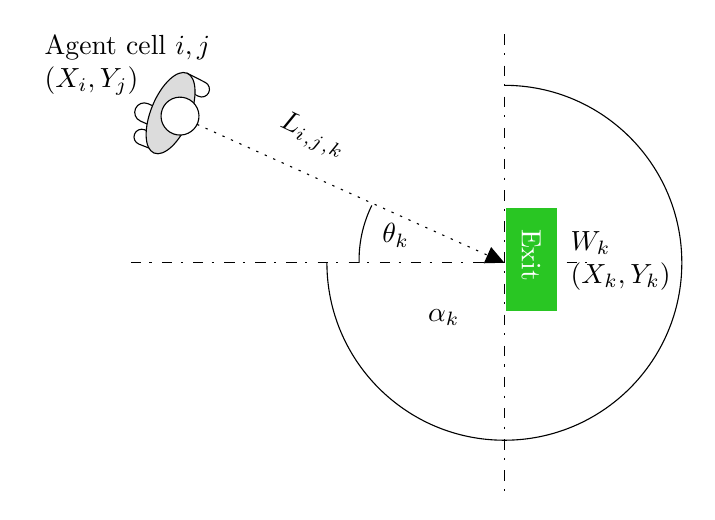
\begin{tikzpicture}[x=0.75pt,y=0.75pt,yscale=-1,xscale=1]

\draw  [fill={rgb, 255:red, 255; green, 255; blue, 255 }  ,fill opacity=1 ] (251.89,35.1) .. controls (253.72,36.03) and (254.45,38.27) .. (253.52,40.1) -- (253.52,40.1) .. controls (252.59,41.93) and (250.36,42.66) .. (248.53,41.73) -- (239.77,37.28) .. controls (239.77,37.28) and (239.77,37.28) .. (239.77,37.28) -- (243.13,30.66) .. controls (243.13,30.66) and (243.13,30.66) .. (243.13,30.66) -- cycle ;
\draw   (219.91,64.83) .. controls (218,64.08) and (217.06,61.93) .. (217.81,60.02) -- (217.81,60.02) .. controls (218.55,58.11) and (220.71,57.16) .. (222.62,57.91) -- (233.06,61.99) .. controls (233.06,61.99) and (233.06,61.99) .. (233.06,61.99) -- (230.35,68.91) .. controls (230.35,68.91) and (230.35,68.91) .. (230.35,68.91) -- cycle ;
\draw   (220.62,53.71) .. controls (218.31,52.69) and (217.27,49.99) .. (218.29,47.69) -- (218.29,47.69) .. controls (219.32,45.38) and (222.01,44.34) .. (224.32,45.36) -- (229.34,47.59) .. controls (229.34,47.59) and (229.34,47.59) .. (229.34,47.59) -- (225.64,55.94) .. controls (225.64,55.94) and (225.64,55.94) .. (225.64,55.94) -- cycle ;
\draw  [draw opacity=0] (396,36.5) .. controls (396,36.5) and (396,36.5) .. (396,36.5) .. controls (396,36.5) and (396,36.5) .. (396,36.5) .. controls (443.22,36.5) and (481.5,74.78) .. (481.5,122) .. controls (481.5,169.22) and (443.22,207.5) .. (396,207.5) .. controls (348.78,207.5) and (310.5,169.22) .. (310.5,122) .. controls (310.5,121.92) and (310.5,121.84) .. (310.5,121.76) -- (396,122) -- cycle ; \draw   (396,36.5) .. controls (396,36.5) and (396,36.5) .. (396,36.5) .. controls (396,36.5) and (396,36.5) .. (396,36.5) .. controls (443.22,36.5) and (481.5,74.78) .. (481.5,122) .. controls (481.5,169.22) and (443.22,207.5) .. (396,207.5) .. controls (348.78,207.5) and (310.5,169.22) .. (310.5,122) .. controls (310.5,121.92) and (310.5,121.84) .. (310.5,121.76) ;  
\draw  [dash pattern={on 0.84pt off 2.51pt}]  (243.88,53.49) -- (267.96,64.34) -- (393.26,120.77) ;
\draw [shift={(396,122)}, rotate = 204.24] [fill={rgb, 255:red, 0; green, 0; blue, 0 }  ][line width=0.08]  [draw opacity=0] (8.93,-4.29) -- (0,0) -- (8.93,4.29) -- cycle    ;
\draw  [draw opacity=0] (326,122) .. controls (325.99,121.62) and (325.99,121.23) .. (325.99,120.85) .. controls (325.99,111.35) and (328.2,102.37) .. (332.12,94.39) -- (385.99,120.85) -- cycle ; \draw   (326,122) .. controls (325.99,121.62) and (325.99,121.23) .. (325.99,120.85) .. controls (325.99,111.35) and (328.2,102.37) .. (332.12,94.39) ;  
\draw  [dash pattern={on 3.75pt off 3pt on 0.75pt off 3.75pt}]  (216,122) -- (436,122) ;
\draw  [fill={rgb, 255:red, 220; green, 220; blue, 220 }  ,fill opacity=1 ] (243.13,30.66) .. controls (247.94,32.64) and (248.27,42.86) .. (243.88,53.49) .. controls (239.49,64.12) and (232.04,71.12) .. (227.23,69.14) .. controls (222.43,67.15) and (222.09,56.93) .. (226.49,46.3) .. controls (230.88,35.68) and (238.33,28.67) .. (243.13,30.66) -- cycle ;
\draw  [fill={rgb, 255:red, 255; green, 255; blue, 255 }  ,fill opacity=1 ] (234.32,43.97) .. controls (238.39,40.99) and (244.11,41.87) .. (247.09,45.94) .. controls (250.08,50.01) and (249.2,55.73) .. (245.13,58.71) .. controls (241.05,61.69) and (235.34,60.81) .. (232.35,56.74) .. controls (229.37,52.67) and (230.25,46.96) .. (234.32,43.97) -- cycle ;
\draw  [dash pattern={on 3.75pt off 3pt on 0.75pt off 3.75pt}]  (396,12) -- (396,232) ;

% Text Node
\draw (336,101.9) node [anchor=north west][inner sep=0.75pt]    {$\theta_k $};
% Text Node
\draw (358,143.4) node [anchor=north west][inner sep=0.75pt]    {$\alpha_k $};
% Text Node
\draw  [color={rgb, 255:red, 255; green, 255; blue, 255 }  ,draw opacity=1 ][fill={rgb, 255:red, 41; green, 198; blue, 35 }  ,fill opacity=1 ]  (396.5,95.5) -- (421.5,95.5) -- (421.5,145.5) -- (396.5,145.5) -- cycle  ;
\draw (409,120.5) node  [rotate=-90] [align=left] {\textcolor[rgb]{1,1,1}{{\fontfamily{helvet}\selectfont  \ Exit \ }}};
% Text Node
\draw (420,103.4) node [anchor=north west][inner sep=0.75pt]    {$ \begin{array}{l}
W_{k}\\
( X_{k} ,Y_{k})
\end{array}$};
% Text Node
\draw (290.8,46.4) node [anchor=north west][inner sep=0.75pt]  [rotate=-25.26]  {$L_{i}{}_{,}{}_{j}{}_{,}{}_{k}$};
% Text Node
\draw (166.6,9) node [anchor=north west][inner sep=0.75pt]    {$ \begin{array}{l}
\mathrm{Agent\ cell} \ i,j\\
( X_{i} ,Y_{j})
\end{array}$};


\end{tikzpicture}

\end{document}